%%
%% This is file `pst-pdf-example1.tex',
%% generated with the docstrip utility.
%%
%% The original source files were:
%%
%% pst-pdf.dtx  (with options: `example1')
%% 
%% This is a generated file.
%% 
%% Copyright (C) 2004-2008 by Rolf Niepraschk <Rolf.Niepraschk@gmx.de>
%%                            and Hubert Gaesslein
%% 
%% This file may be distributed and/or modified under the conditions of
%% the LaTeX Project Public License, either version 1.2 of this license
%% or (at your option) any later version.  The latest version of this
%% license is in:
%% 
%%    http://www.latex-project.org/lppl.txt
%% 
%% and version 1.2 or later is part of all distributions of LaTeX version
%% 1999/12/01 or later.
%% 
%% Process this file with the scripts `ps4pdf' or `ps4pdf.bat' or call
%%
%%   latex pst-pdf-example1.tex
%%   dvips -Ppdf -o pst-pdf-example1-pics.ps pst-pdf-example1.dvi
%%   ps2pdf -dAutoRotatePages=/None pst-pdf-example1-pics.ps pst-pdf-example1-pics.pdf
%%   pdflatex pst-pdf-example1.tex
%%
\listfiles
\documentclass[12pt,a4paper]{article}
\usepackage[margin={25mm,30mm}]{geometry}

\usepackage[dvipsnames]{pstricks}
\usepackage{pst-node,pst-tree,psfrag}
\usepackage{pst-pdf}

\pagestyle{empty}

\begin{document}

\section*{\textsf{pst-pdf:} A short example document}

\subsection*{png graphic and postscript graphic together}

\noindent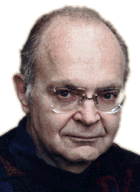
\includegraphics[width=.35\textwidth]{knuth}% A none-ps graphic
\hfill

\includegraphics[width=.60\textwidth]{elephant}%       A ps graphic

\subsection*{PSTricks code inside a pspicture environment}

\newpsobject{showgrid}{psgrid}{subgriddiv=1,griddots=10,gridlabels=8pt}

\begin{center}
\begin{pspicture}(-5.25,-5.25)(5.25,5.25)%
  \pscircle*[linecolor=Apricot]{5}
  \rput(0,0.5){
\includegraphics[width=8\psxunit]{elephant}}
  \Huge\sffamily\bfseries
  \rput(-4.5,4.5){A} \rput(4.5,4.5){B}
  \rput(-4.5,-4.5){C}\rput(4.5,-4.5){D}
  \rmfamily
  \rput(0,-3.8){PSTricks}
  \rput(0,3.8){\LaTeX}
  \showgrid
\end{pspicture}
\end{center}

\subsection*{PSTricks code without a pspicture environment}

%%----------------------------------------------------------------------
%% From: The \LaTeX\ Graphics Companion; first release.
\definecolor{pink}{rgb}{1, .75, .8}
\renewcommand\psedge{\nccurve}
\newcommand{\Female}[2][]{{\psset{linecolor=pink}\TR[#1]{\emph{#2}}}}
\newcommand{\Male}[2][]{{\psset{linecolor=blue}\TR[#1]{#2}}}
\psset{nodesep=2pt,angleA=90,angleB=-90}
\footnotesize

\pstree[treemode=U]{\Female{{\bfseries Matilde}}}{%
  \pstree{\Male{Sebastian}}{%
    \pstree{\Male[name=P]{Philip}}{\Male{Frederick}\Female{Ethel}}
    \pstree{\Female[name=W]{Mary}}{\Male{Lionel}\Female{Agnes}}}
  \pstree{\Female{Leonor}}{%
    \pstree{\Male[name=R]{Ra\'ul}}{\Male{Joaquim}\Female{J\'ulia}}
    \pstree{\Female[name=A]{Am\'elia}}{\Male{\'Alvaro}\Female{Augusta}}}
}

%%----------------------------------------------------------------------

\subsection*{psfrag demo}

\normalsize

\noindent

\includegraphics[width=.475\textwidth]{psf-demo.eps}
\hfill
\begin{psfrags}
  \psfragscanon
  \psfrag{x1}[br][  ]{\LaTeX} \psfrag{x2}[br][br]{\LaTeX}
  \psfrag{x3}[br][tl]{\LaTeX} \psfrag{x4}[br][Br]{\LaTeX}
  \psfrag{x5}[Br][ r][1.15][45]{\Huge\LaTeX}
  \psfrag{x6}[tl][ l][1.15][45]{\Huge\LaTeX}
  
\includegraphics[width=.475\textwidth]{psf-demo}
\end{psfrags}

\subsection*{The postscript environment}

\begin{center}
\begin{postscript}
\Large
\noindent
$
  \bordermatrix{%
  & A            & B & C\cr
  & \rnode{D}{D} & E & \rnode{F}{F}\cr
  & G            & H & I\cr
  & \rnode{J}{J} & K & M
  }
$
\ncline[nodesep=-1em,linecolor=red]{D}{F}
\ncline[nodesep=-1em,linecolor=red]{D}{J}
\end{postscript}
\end{center}

\end{document}
\endinput
%%
%% End of file `pst-pdf-example1.tex'.
